%\documentclass[6pt, twocolumn]{ctexart}
\documentclass[10pt, twocolumn]{ctexart}
%\documentclass[10pt,conference,letterpaper]{IEEEtran}
%\usepackage{multicol}
\usepackage{float}
\usepackage{color}
\usepackage{CJK}
\usepackage{array}
\usepackage{rotating}   % 图片旋转 
\usepackage{subfigure}
\usepackage{graphicx}   % 插图必用宏包 
\usepackage{biblatex}
\usepackage{amsmath}
\usepackage{algorithmic}
\usepackage{algorithm}
\bibliography{sample}
\renewcommand{\abstractname}{摘 要}  % 将Abstract改为摘要
\renewcommand{\refname}{参考文献}   % 将References改为参考文献
\renewcommand{\indexname}{索引}
\renewcommand{\figurename}{图}
\renewcommand{\tablename}{表}
\renewcommand{\appendixname}{附录}
\begin{document}


\title{全排列生成算法的研究与优化}
\author{秦雪迪\footnote{秦雪迪 2017310722 qxd17@mails.tsinghua.edu.cn } 、 仝美涵\footnote{仝美涵 2017310729  tongmh17@mails.tsinghua.edu.cn} 、
田冰\footnote{田冰 2017310757 tb17@mails.tsinghua.edu.cn}  \\ 清华大学计算机科学与技术系软件所}
\date{}
\maketitle

\begin{abstract}全排列生成问题指的是对于$n$个相互不同的元素,如何输出这$n$个元素所有不同的排列。本文研究并实现了字典序法、利用中介数产生全排列的字典序法、递增进位制法、递减进位制法以及邻位对换法,并通过实验对这五种算法的效率和复杂度进行了分析。同时,在这五种算法的基础上,结合动态规划和二叉树的思想,提出了三种优化求解中介数的算法,同时利用中介数未进位的特殊性,对生成后续排列的过程进行了优化。实验结果表明,我们的优化能够显著提高全排列算法的性能。 
\end{abstract}

\section{引言}组合数学是一门研究离散对象的科学,是计算机科学的基础。随着计算机的应用越来越普及,组合数学的研究将更加深入。其最主要的研究内容就是对离散对象的计数\cite{卢开澄2006组合数学}。学习组合数学的基础就是排列组合。排列是指从多个不同元素中取出几个元素按照一定顺序排成一列的过程,排列的种类数称为排列数,用$P_{n}^m$表示。组合是指从多个不同元素中取出元素组成一个集合的过程,组合的种类数称为组合数,用$C_n^m$表示。
全排列的生成算法是将给定的序列中所有可能的全排列无重复无遗漏地枚举出来。此处全排列的定义是:从$n$个元素中取出$m$个元素进行排列,当$n=m$时这个排列被称为全排列。字典序、邻位对换法、递增进位制法、递减进位制法都是常见的全排列生成算法。全排列生成算法有广泛的应用,例如可以应用在不同的组合优化问题(例如TSP问题)、$n$皇后问题、克莱姆法则\cite{李模刚2010全排列生成算法在克莱姆法则中的应用}、图论问题(例如图同构问题)等的算法设计中\cite{Maccallum1977Surveyor}。针对全排列的生成,Robert Sedgewick在1997年写了一份全排列生成算法的调查报告\cite{Sedgewick1977Permutation},对当时几乎全部的全排列生成算法做了比较,并得出一个结论:Heap提出的全排列生成算法在大多数情况下是最快的。C++的STL中定义的next\_permutation和prev\_permutation函数也是十分灵活高效的算法,被广泛应用于为指定序列生成后一个和前一个排列。除此之外,还有一类利用中介数和排列一一对应的关系,从而利用中介数生成全排列的算法,例如,字典序全排列,递增进位制法,递减进位制法以及邻位对换法等。

本文即是针对这几种算法,进行研究和改进。本文的工作如下:\\
\begin{itemize}
  \item 实现了五个全排列生成算法同时对算法效率和复杂度进行了分析;
  \item 利用中介数未进位的特殊性,对生成后续排列的过程进行了优化,并通过实验比较优化前后的算法效率;
  \item 利用基于动态规划和不同特点的二叉树的思想,提出了三种优化求解中介数的算法,并通过实验比较优化前后的算法效率; 
\end{itemize}
\section{相关工作}
\subsection{字典序法}
设 $P$ 是 $1\sim n$ 的一个全排列,$P=p_1p_2\cdots p_n$。字典序法就是按照字典序依次求出下一个排列的算法。这要求相邻的两个字典有尽可能长的共同前缀,将变化限制在尽可能短的后缀上。具体方法如下:
\begin{enumerate}
  \item 从排列的右端开始,找出第一个比右边数字小的数字的位置$j$
  \item 找出在$p_j$右边的数字中,比$p_j$大的数中最小的数字$p_k$
  \item 交换$p_j$和$p_k$,将序列$p_{k+1}\sim p_{n}$倒转即可以得到下一个序列
\end{enumerate} 

除此之外,字典序法也可以通过中介数进行计算。中介数是计算排列的中介环节,它的每一位由原排列每个数字右侧比其小的数字个数构成。 其运 算过程为:原排列→中介数→新中介数→新排列。

设得到的新中介数位$b = b_n\cdots b_{2}$,要求的排列为$r= r_n\cdots r_1$。\\
\textbf{算法流程:}
中介数初始值每一位都是$0$,根据中介数,从高位到低位依次遍历中介数从而确定排列的每一位,若当前中介数中第$i$位的值为$b_i$,就在剩余的还没有被排过的数中找出第$b_i+1$小的数,那么$r_i$就等于这个数。依次遍历完中介数的每一位后,还没被排过的数即为$r_1$位对应的数。由此,一个新的排列生成。中介数加$1$,根据上述算法产生下一个排列。直到中介数最高位等于产生进位,算法结束,所有的字典序全排列都已生成。
\subsection{递增进位制法}
人们通常所用的进制大多是固定进位制,如$2$进制,$10$进制等。$m$位$n$进制可以表示的数字个数为 $m^n$个。而递增/递减进位制数,顾名思义,是指数 字的进制随着数字位置的不同递增/递减的进制。$m$ 位递增/递减进位制数可以表示$m!$数字。例如递增进位制$4121$,它的进制从右向左依次为 $2$,$3$,$4$,$5$, 换算成十进制相当于数字$107$。

递增进位制法生成全排列可以通过中介数进行计算。设中介数位$b = b_n\cdots b_{2}$,$b_i$表示在排列中i这个数字右边比i小的数有$b_i$个,假设要求的排列为$r= r_n\cdots r_1$。\\
\textbf{算法流程:}
中介数初始值每一位都是$0$,根据中介数,从高位到低位依次遍历中介数从而确定排列的每一位,若当前中介数中第$i$位的值为$b_i$,则从右向左扫描所有没有被排过数字的位置,直到第$b_i+1$个位置$j$,那么$i$就在这个位置上,即$r_j=i$。依次遍历完中介数的每一位后,还没被排过的位置即为$1$所在的位置。由此,一个新的排列生成。中介数加$1$,根据上述算法产生下一个排列。由此,一个新的排列生成。中介数按照递增进位制加法加1,根据上述算法产生下一个排列。直到中介数最高位等于产生进位,算法结束,所有的递增进位制法全排列都已生成。
\subsection{递减进位制法}
在通过递增进位制的加法生成下一个中介数时,由于递增进位制越低位进制越小,所以在加法的过程中极易产生进位,算法效率受到了限制,因此,提出了一种新的算法:递减进位制法。和递增进位制法不同,递减进位制越高位进制越小。在通过中介数生成全排列时,算法流程与递增进位制法类似。\\
\textbf{算法流程:}
设中介数位$b = b_2\cdots b_{n}$,$b_i$表示在排列中i这个数字右边比i小的数有$b_i$个,假设要求的排列为$r= r_n\cdots r_1$。中介数初始值每一位都是$0$,根据中介数,从低位到高位依次遍历中介数从而确定排列的每一位,若当前中介数中第$i$位的值为$b_i$,则从右向左扫描所有没有被排过数字的位置,直到第$b_i+1$个位置$j$,那么$i$就在这个位置上,即$r_j=i$。依次遍历完中介数的每一位后,还没被排过的位置即为1所在的位置。由此,一个新的排列生成。中介数按照递增进位制加法加$1$,根据上述算法产生下一个排列。直到中介数最高位等于产生进位,算法结束,所有的递减进位制法全排列都已生成。
\subsection{邻位对换法}
递增进位制和递减进位制数字的换位是单向的,而邻位对换法的换位是双向的,通过保存数字的``方向性"来快速得到下一 个排列。\\
\textbf{算法流程:}
设中介数位$b = b_2\cdots b_{n}$,$b_i$表示在排列中$i$这个数字右边比i小的数有$b_i$个,假设要求的排列为$r= r_n\cdots r_1$。由中介数得到排列时,假设第$b_k$位的值为$i$,方向是向左的,就从右向左扫描所有没有被占过的位置,知道第$b_i+1$位置$j$,那么$i$就在这个位置上,即$r_j=i$。如果方向是向右的,那么转化成向左的进行计算,即表示$i$的左边比$i$小的数有$b_i$个 也即相当于i的右边比i小的数有$i-1-b_i$个。依次遍历完中介数的每一位后,还没被排过的位置即为1所在的位置。由此,一个新的排列生成。中介数按照递增进位制加法加$1$,根据上述算法产生下一个排列。直到中介数最高位等于产生进位,算法结束,所有的临位对换法全排列都已生成。

\section{算法效率和时间复杂度分析}
\subsection{时间复杂度分析}
$n$个数字的全排列一共有$n!$种,所以全排列算法至少是$O(n!)$的。字典序算法在生成下一个排列时需要扫描全排列找出第一个下降的数字并交换,因此字典序算法的时间复杂度是$O(n*n!)$;采用中介数的字典序法、递增进位制数法、递减进位制数法和邻位对换法在求下一个全排列时,需要先生成中介数,而生成中介数的时间复杂度是$O(n^2)$,因此它们的时间复杂度是$O(n^2*n!)$。所以实际上,全排列算法对大型的数据是无法处理的。也正因为如此,研究如何降低全排列生成算法的时间复杂度是非常重要的。


\subsection{几种全排列生成算法的效率分析}
本节我们比较了字典序算法(DIC1)以及基于中介数的字典序算法(DIC2)、递增进位制法(INCRE)、递减进位制法(DIM)以及邻位对换法(EXCHANGE)这五种算法在生成全部排列方面的性能,如图\ref{quan_experiment} 所示。
\begin{figure}[H]
\centering
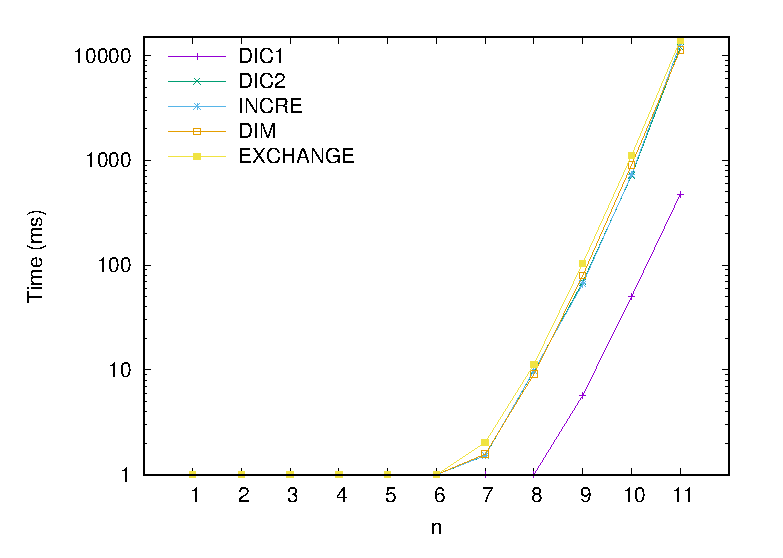
\includegraphics[width=1\columnwidth]{pictures/quan.eps}
\caption{全排列生成算法比较}
\label{quan_experiment}
\end{figure}

从图中可以看出,不使用中介数的字典序算法是五种算法中最快的算法,而使用中介数的邻位对换法是五种算法中最慢的算法。当排列的位数超过$10$后,使用中介数的四种算法性能急剧下降,这是因为由排列得到中介数和由中介数得到排列的计算次数急剧增加。可见当位数较大时,使用中介数作为媒介会大大降低全排列生成算法的性能。


\section{ 利用中介数未进位的特殊性生成后续排列 }
\subsection{特殊性分析}
在四种算法中,如若我们希望求当前排列数$P$的后第$A$个排列数,在中介数没有发生进位的情况下,我们可以通过移动原排列数的若干位,直接生成新的排列数。

\iffalse
设$P$是$1\sim n$的一个全排列,$P=p_1p_2\cdots p_n$,那么定义$C$:
\begin{displaymath}
C=c_1c_2\cdots c_n
\end{displaymath}
\begin{equation}
c_i=\|\{x < p_i\mid x\in\{p_1p_2\cdots p_{i-1}\}\|
\end{equation}
设A对应的字典序进制下的数a为
\begin{displaymath}
a=a_1a_2\cdots a_n-1
\end{displaymath}
那么,当$a$满足下述式子时,$P$生成新排列的过程中中介数不会发生进位。
\begin{equation}
a_i\leq c_i 
\end{equation}
\begin{displaymath}
0\leq i\leq n
\end{displaymath}
同理,求排列数$P$的前第$A$个排列数时,中介数不发生变化的条件是
\begin{equation}
c_i=\|\{x < p_i\mid x\in\{p_{i+1}p_{i+2}\cdots p_n\}\|
\end{equation}
\begin{equation}
a_i\leq c_i 
\end{equation}
\begin{displaymath}
0\leq i\leq n
\end{displaymath}
\fi

设$P$是$1\sim n$的一个全排列,$P=p_1p_2\cdots p_n$,数组$I$存储排列中每个数字的下标,则$I_{i}$表示数字$i$在排列$P$中的位置。定义$C$为:
\begin{displaymath}
C=c_1c_2\cdots c_n
\end{displaymath}
\begin{equation}
c_i=|\{x < i\mid x\in\{p_1p_2\cdots p_{I_i-1}\}|
\end{equation}
设$A$对应的递减进制下的数为$a=a_1a_2\cdots a_{n-1}$,那么若$\forall i\in[1,n]$,$a_i \leq c_i$都成立,则$P$生成新排列的过程中中介数不会发生进位。同理,求排列$P$的前第$A$个排列数时,中介数不进位的条件是$\forall i\in[1,n]$,$a_i\leq c_i$都成立,其中$c_i=|\{x < i\mid x\in\{p_{I_i+1}p_{I_i+2}\cdots p_n\}|$。



下述算法是在该条件成立下计算新排列数的。
\subsection{算法介绍}
该算法省去了生成中介数的过程,可以直接根据原排列$P$和改变量$A$,求出新的排列数,具体流程如下:
\begin{enumerate}
  \item 遍历排列数$P$,计算$C$,并将$2\sim n$所处位置的下标记录在位置数组$I$中
  \item 根据选择的算法,将$A$转换位递增进制数或者递减进制数
  \item 判断$A$与$C$是否满足公式(1)中所给的条件。若不满足,则终止算法
  \item 从后向前遍历$I$,假设当前遍历到$I$的第$i$位$I_i$
  \item 根据$I_i$中记录的位置信息,找到数字$i+2$在原排列中的位置
  \item 从数字$i+2$开始,与比其小的数字交换$a_i$次,求出该数字在新排列中的位置
  \item 当$i$等于0时结束算法 
\end{enumerate} 
\subsection{优化算法性能分析}
上述流程中,前三步的时间复杂度都为$O(n)$,后三步时间复杂度近似于$O(n^2)$,虽然与传统算法的时间复杂度一致,但是与其相比,该算法省去了生成中介数,再反向生成新排列的过程,在实际的实验中我们可以看到明显的速度提升。

\iffalse
实现该算法需要存储数组$P$,$A$,$N$,他们的长度分别为n,n-2,n-2,因此该算法的空间复杂度为O(n),可以看到与传统的递减进制数算法相比算法多出了$N$,$C$这两个数组,少了存储新排列的数组,但是整体来说两者的空间复杂度是一致的。
\fi




\section{基于动态规划生成中介数}
基于中介数的四种全排列生成算法的时间复杂度为$O(n^2*n!)$,其中求解中介数的时间复杂度为$O(n^2)$。以字典序为例,当$n=100000$时, 仅求解中介数就需要大约$24s$,这是十分耗时 的。因此本节和下一节提出了两种优化求解中介数的算法:基于动态规划和二叉树生成中介数的算法。本节将详细介绍基于动态规划生成中介数的算法思想。
\iffalse
在很多应用场景下,我们需要求出某个排列后面的第$m$个排列。\textcolor{red}{比如...?}设原排列为$P$,目标排列即原排列的后续第$m$个排列为$\bar{P}$。在字典序法,递增进位制法,递减进位制法和邻位对换法中求$\bar{P}$的方法一般为首先找到原排列的中介数$A$,然后将中介数加$m$得到新的中介数$\bar{A}$,依据新的中介数找到目标排列。本节基于动态规划的思想,提出了一种优化求解中介数的算法,该算法在一般情况下可以优化一般算法$3-3.5$倍时间。

\subsection{求后续排列的一般算法}
以字典序算法为例,算法\ref{next_permutation} 给出了求目标排列的基本流程。首先通过GET\_AGENCY函数获取原排列$P$的中介数$A$,将$m$按照中介数进制(从左到右每位的进制依次是$n,n-1,...,2$)表示,得到$A_m$(第3-6行)。然后将$A$和$A_m$相加,得到$\bar{A}$(第7-17行)。最后根据新的中介数$\bar{A}$求出目标排列$\bar{P}$。
\begin{algorithm}[!t]
\caption{NEXT\_PERMUTATION (P,m,n)}
\label{next_permutation}
\begin{algorithmic}[1]
\STATE $A=$ GET\_AGENCY$(P,n)$
\STATE {$A_m,\bar{A},\bar{P} \leftarrow [0]$}
\FOR{$i \leftarrow n-1$ to $1$} 
\STATE {$A_m[i] \leftarrow m\%(n+1-i)$}
\STATE {$m \leftarrow m/(n+1-i)$}
\ENDFOR
\STATE {$flag,tmp \leftarrow 0$}
\FOR{$i \leftarrow n-1$ to $1$} 
\STATE {$tmp \leftarrow A[i]+A_m[i]+flag$}
\IF{$tmp\ge n+1-i$}
\STATE {$\bar{A}[i] \leftarrow tmp-(n+i-i)$}
\STATE {$flag \leftarrow 1$}
\ELSE
\STATE {$\bar{A}[i] \leftarrow tmp$}
\STATE {$flag \leftarrow 0$}
\ENDIF
\ENDFOR
\STATE calculate $\bar{P}$ from $\bar{A}$
\RETURN $\bar{P}$
\end{algorithmic}
\end{algorithm}




\subsection{求中介数的一般算法}
在字典序算法中,中介数$A[i]$表示$P[i]$右边比$P[i]$小的数字的个数。算法\ref{get_agency} 给出了求解中介数的一般算法。该算法包括两层循环,外层循环遍历排列中的每一个数,内层循环找出这个数对应的中介数,即找出该数右侧比它小的数字个数。因此算法\ref{get_agency} 的时间复杂度为$O(n^2)$。当$n=100000$时,仅求解中介数就需要大约$24s$,这是十分耗费时间的。因此改进中介数的求解算法是十分必要的。

\begin{algorithm}
\caption{GET\_AGENCY (P,n)}
\label{get_agency}
\begin{algorithmic}[1]
\STATE {$A \leftarrow [0]$}
\FOR{$i \leftarrow 1$ to $n-1$} 
\FOR{$j \leftarrow i+1$ to $n$} 
\IF {$P[j]<P[i]$}
\STATE {$A[i] \leftarrow A[i]+1$}
\ENDIF
\ENDFOR
\ENDFOR
\RETURN $A$
\end{algorithmic}
\end{algorithm}
\fi


\subsection{原理分析}
以字典序为例,通过观察中介数的求解过程,我们得到了两个重要的结论:
\begin{enumerate}
  \item 当求解排列中数字$i$的中介数时,设$i$左右两侧排列分别为$P1$,$P2$,若$i$左侧数字个数小于右侧数字个数,即$|P1|<|P2|$,那么扫描$P1$中比$i$小的数字个数可以更快的得到$i$的中介数;
  \item 设$i$与$i+1$之间的排列为$P3$,若已知$i+1$的中介数,且$i$与$i+1$在$P$中距离很小,那么可以通过$i+1$的中介数快速求解出i的中介数;
\end{enumerate}
设$P=P[1],P[2],...,P[n]$,数组$A$存储排列中每个数字对应的中介数,即$A[i]$为$P[i]$的中介数;数组$I$存储排列中每个数的下标,即$I_{i}$表示数字$i$在排列$P$中的位置。综合以上观察,在求解排列中数i的中介数时,由于$i$在$P$中的位置为$I[i]$,故$P1=P[1:I[i]]$,$P2=P[I[i]+1:n]$,$P3=P[I[i]:I[i+1]]$,令$P_{min}=min(P1,P2,P3)$,即$P1$,$P2$,$P3$中最短的一段,通过扫描$P_{min}$中比$i$小的数字个数(设为$t$)来计算$i$的中介数,即$A[I[i]]$,可以有效缩短计算中介数的时间。当$P1$最短时,$t$为$i$左侧比$i$小的数字个数,而比$i$小的数字个数共有$i-1$个,故$A[I[i]]=i-1-t$;当$P2$最短时,$A[I[i]]=t$;当$P3$最短时,若$i$位于$i+1$左侧,即$P=\cdots i \cdots i+1 \cdots$,由于比$i+1$小的数都会比i小,故而$i$的中介数等于$t$加上$i+1$的中介数,若$i$位于$i+1$的右侧,即$P=\cdots i+1\cdots i \cdots$,则$i$的中介数等于$i+1$的中介数减去$1+t$。算法\ref{get_agency_optimization} 展示了这一过程。

\iffalse
\begin{equation}
A[I[i]]=\left\{
\begin{array}{ll}
i−1−A[I[i]] &  S1=S         \\
A[I[i]]     &  S2=S   \\
A[I[i+1]]+A[I[i]]  & S3=S  \\
\end{array}\right.
\end{equation}

\begin{equation}
A[I[i]]=\left\{
\begin{array}{ll}
i−1−A[I[i]] &  S1=S         \\
A[I[i]]     &  S2=S   \\
A[I[i+1]]−A[I[i]]−1  & S3=S  \\
\end{array}\right.
\end{equation}
\fi


\begin{algorithm}[!t]
\caption{DP (P,n)}
\label{get_agency_optimization}
\begin{algorithmic}[1]
\STATE calculate $I$ from $P$
\STATE calculate $A[I[n]]$
\FOR{$i \leftarrow n-1$ to $1$} 
\STATE {$P1 \leftarrow P[1:I[i]]$}
\STATE {$P2 \leftarrow P[I[i]+1:n]$}
\STATE {$P3 \leftarrow P[I[i]:I[i+1]]$}
\STATE {$P_{min} \leftarrow min(P1,P2,P3)$}
\STATE {$t \leftarrow$ the number of numbers in $P_{min}$ smaller than $i$}
\IF {$P1=P_{min}$}
\STATE {$A[I[i]] \leftarrow i-1-t$}
\ELSIF {$P2=P_{min}$}
\STATE {$A[I[i]] \leftarrow t$}
\ELSE 
\IF {$I[i]<I[i+1]$}
\STATE {$A[I[i]] \leftarrow A[I[i+1]]+t$}
\ELSE
\STATE {$A[I[i]] \leftarrow A[I[i+1]]-t-1$}
\ENDIF
\ENDIF
\ENDFOR
\RETURN $A$
\end{algorithmic}
\end{algorithm}
\subsection{优化算法性能分析}
优化算法每次扫描的排列序列为$P1$,$P2$,$P3$中最短的一段,因此从理论上来说优化算法可以有效减少求中介数的时间。而且当排列较为均匀,即$\sum_{i=1}^{n-1}\left|I[i]-I[i+1]\right|$较小时(比如$P=1,2,3,...,n$),由于$P3$很小,优化算法可以在接近$O(n)$的时间内求出排列的中介数。




\section{ 利用二叉树生成中介数}
\subsection{原理分析}
当我们从排列数生成中介数时,实际是在求每位数字在排列数中右边比它小的数的个数,那么我们可以从右向左构建二叉树来优化这一过程。
设$P$是$1\sim n$的一个全排列,$P=p_1p_2\cdots p_n$,设$A$是$P$对应的中介数,$A=a_1a_2\cdots a_{n-1}$。树中每个结点T由以下三个元素构成:

\begin{tabular}{m{1cm} l m{8cm}}
\\
$d$ & 记录排列数 \\
$l$ & 记录左孩子的数目\\ 
$m$ & 记录排列数对应的中介数\\
\\
\end{tabular}

这里我们以递减进位制为例来说明我们的算法,递增进位制,字典序进位制类似。

我们从$p_n\sim p_1$自后向前依次计算中介数。假设当前计算到$p_i$的中介数$a_{i-1}$,那么我们先利用$p_i$构建一个树的结点$T_i$,从树根$T_0$开始,将$T_i$依次与树中的结点比较。
假设我们比较到第$k$个结点$T_k$,如果$T_k$中存储的排列数比$T_i$存的小,则走左岔路,并更新$T_k$左孩子的个数;如果结点$T_k$中存储的排列数比$T_i$存的大,则走右岔路,并更新$T_i$的中介数。一旦$T_i$到达叶结点,则终止算法。其中左孩子和中介数的更新规则为$l_k= l_k + 1$,$m_i = m_i + l_k + 1$。
\iffalse
\begin{equation}
l_k= l_k + 1
\end{equation}
\begin{equation}
m_i = m_i + l_k + 1
\end{equation}
\fi

图\ref{example1} 展示了排列``361452"生成中介数的过程。其中每个结点存储两个信息,第一个为该节点的左孩子数,第二个为该节点对应的中介数。可以看到每插入一个结点,根据该节点第二个中介数信息,就能够立刻得到该结点对应的中介数。
\begin{figure}[!t]
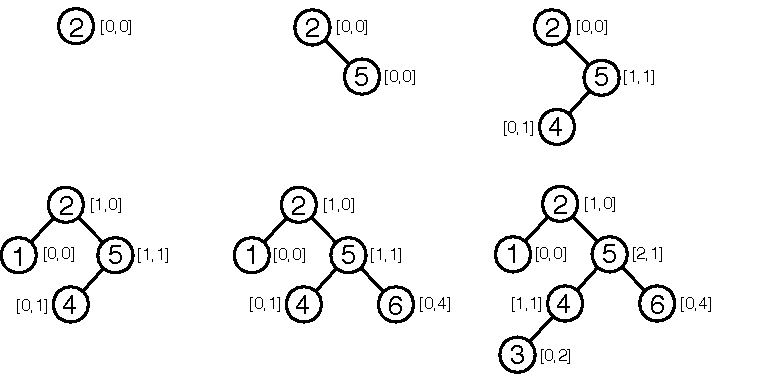
\includegraphics[width=1\columnwidth]{pictures/example1.pdf}
\caption{利用二叉树生成中介数}
\label{example1}
\end{figure}


\subsection{利用平衡二叉树进一步优化算法}
可以看到,上述算法构建的树并不平衡,这会导致插入效率降低,为了更好的时间性能,我们引用了AVL平衡二叉树\cite{Adel1962An}。
我们将树的节点重新定义如下:

\begin{tabular}{m{1cm} l m{8cm}}
\\
$d$ & 记录排列数 \\
$l$ & 记录左孩子的数目\\ 
$r$ & 记录右孩子的数目\\
$a$ & 记录左树的深度\\
$b$ & 记录右树的深度\\
$m$ & 记录排列数对应的中介数\\
\\
\end{tabular}

图\ref{example2} 显示了排列``361452"在平衡二叉树上的计算流程。每插入完一个节点,自底向上地采用单旋或者双旋的方法,调整一次树,保证每个节点左右树深之差不超过1,使得算法的效率得到进一步的提高。
\begin{figure}[H]
\centering
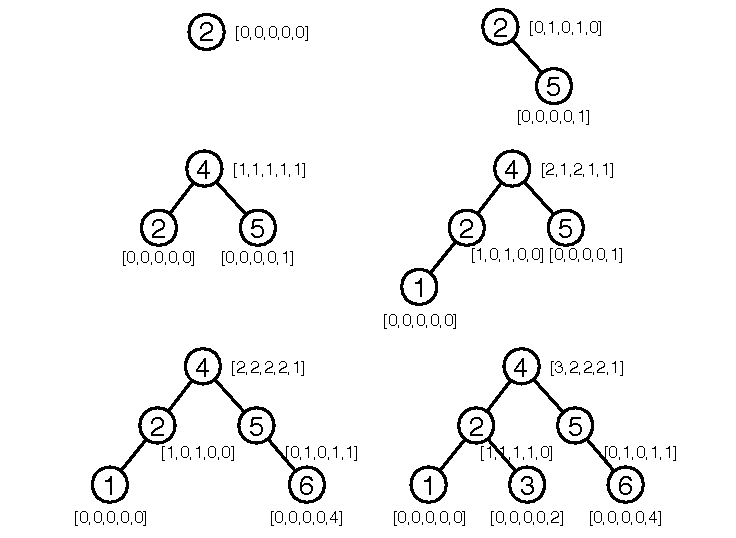
\includegraphics[width=0.9\columnwidth]{pictures/example2.pdf}
\caption{利用平衡二叉树生成中介数}
\label{example2}
\end{figure}
\subsection{优化算法性能分析}
可以看到,我们需要从右向左依次寻找中介数,该过程为$O(n)$。而寻找中介数的过程实际为$p_i$插入二叉树的过程,该过程的时间复杂度为$O(log(n))$。因此,最终算法的时间复杂度为$O(n*log(n))$。可以看到相比于传统算法$O(n^2)$的复杂度,该算法的复杂度更低,后续实验也证实了该算法的时间优越性。



\section{实验}
为了对优化算法进行性能分析,我们设计了一系列实验来进行测试。本文的所有实验都是在一个16GB内存,2.5GHZ的Intel Core i7处理器的Macbook Pro上进行的。
\subsection{利用中介数未进位的特殊性生成后续排列}
我们依次令$n$取不同的值,随机生成排列$P$和一个满足算法条件的正整数$a$,分别使用递减进位制算法和优化的算法求解$P$的后第$a$个排列,记录计算时间,得到图\ref{teshu} 。由图可知,优化算法省去了大量不必要的计算,极大缩短了计算时间。
\begin{figure}[H]
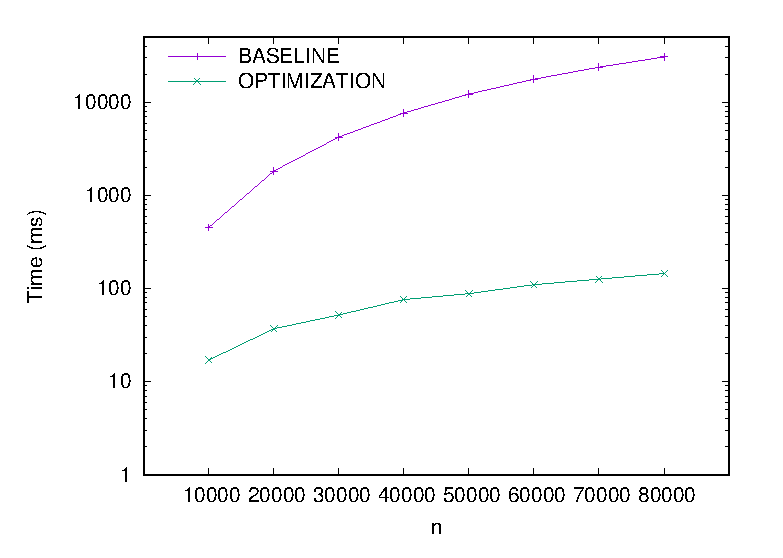
\includegraphics[width=1\columnwidth]{pictures/teshu.eps}
\caption{后续排列优化算法性能分析}
\label{teshu}
\end{figure}
%\iffalse
%总的来说,该算法可以在以下两个场景中极大的提高算法的效率。
%\begin{itemize}
%  \item 生成$1\sim n$的所有全排列。
%  \item 从排列$P$直接生成后第$a$个排列,或者前第$b$个排列。
%\end{itemize} 
%\fi
\subsection{生成中介数的对比实验}
我们依次令$n$取不同的值,以字典序为例,比较生成中介数的常规算法(BASELINE),动态规划算法(DP),二叉树算法(BINARY\_TREE),平衡二叉树算法(AVL)对随机生成排列和均匀排列的运行时间。其中均匀排列即为$\sum_{i=1}^{n-1}\left|I[i]-I[i+1]\right|$较小的排列,实验中取$P=1,2,3,\cdots,n$。
\iffalse

图\ref{agency_experiment} 给出了利用常规算法和优化算法求中介数的实验结果。和常规的递减进位制算法生成中介数相比,三种优化算法均提高了生成中介数的效率。对于基于动态规划的算法,当$n<1000$时,GET\_AGENCY和GET\_AGENCY\_OPTIMIZATION的性能所差无几,而当$n>1000$后,优化算法大致可以加速一般算法$3-3.5$倍。对于基于二叉树的算法,当$n=1^4$时,普通二叉树算法的速度是传统算法的100倍,当$n=1^5$时,普通二叉树算法的速度是传统算法的700倍,并且随着n的增加,加速的效果愈加显著。

同时,我们观察到,三种优化算法对于分布特点不同的原排列,其优化能力是不同的。由图可看出,基于动态规划的算法对均匀数据的优化能力最强,因为它每次扫描的排列序列为$P1$,$P2$,$P3$中最短的一段,因此当排列较为均匀,即时(比如$P=1,2,3,...,n$),由于$P3$很小,优化算法可以在接近$O(n)$的时间内求出排列的中介数。基于二叉树的算法对非均匀数据的优化能力最强,每插入一个结点,根据该节点第二个中介数信息,就能够立刻得到该结点对应的中介 数,该过程的时间复杂度近似为 log(n)。而基于平衡二叉树的优化算法在均匀数据和非均匀数据上都有较好的性能,表现非常稳定。
\fi
\begin{figure}[!t]
\centering
\subfigure[随机数据]{
\label{random_agency}
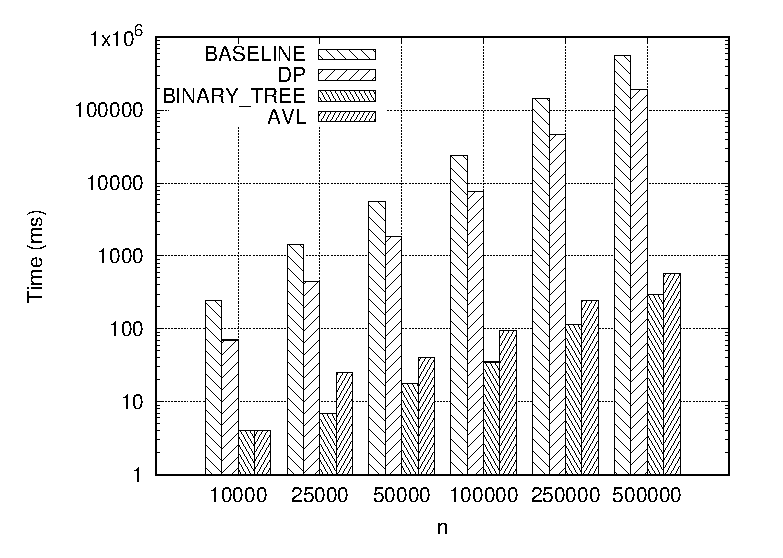
\includegraphics[width=1\columnwidth]{pictures/random_agency.eps}}
\subfigure[均匀数据]{
\label{even_agency}
\includegraphics[width=1\columnwidth]{pictures/even_agency.eps}}
\caption{中介数优化算法性能分析}
\label{agency_experiment}
\end{figure}

图\ref{agency_experiment} 给出了利用常规算法和优化算法求中介数的实验结果。可以看到,对于随机数据,三种优化算法均提高了生成中介数的效率。从优化效果上来看,BINARY\_TREE $>$ AVL $>$ DP。由于基于二叉树的中介数求解算法效率较原算法有量级提升(由$O(n^2)$到$O(n*log(n))$),故其效率远高于DP算法;而DP算法大致可以加速一般算法$3 \sim 3.5$倍。由于数据随机,使得非平衡二叉树也基本处于平衡的状态,故BINARY\_TREE算法整体上优于AVL算法。

对于均匀数据,可以看到DP算法是三种优化算法中最快的,由于数据较为均匀,故而算法时间复杂度接近$O(n)$。而BINARY\_TREE算法不仅没有加速常规算法,反而使得效率变低。这是由于此时二叉树处于极度不平衡状态,基本接近于线性查询,故而效率变低。但此时AVL算法和随机数据时性能基本保持一致。

综合以上分析,我们可以得出以下结论:1)AVL算法在随机数据和均匀数据上都有较好的性能,表现相对稳定,可以应用于对算法稳定性要求较大的场景;2)若数据较为均匀,采用DP算法可以有更好的加速效果;反之,采用BINARY\_TREE算法可以得到更好的结果。因此在求解中介数之前,可以通过判断$\sum_{i=1}^{n-1}\left|I[i]-I[i+1]\right|$的值来决定采用何种算法。



\section{总结与展望}
本文深入研究了全排列的五种经典算法,普通字典序法,基于中介数的字典序法、递增进位制数法,递减进位制法和邻位对换法,并对比了其算法效率。同时,在这五种算法的基础上,结合动态规划和二叉树的思想,提出了三种优化求解中介数的算法。除此之外,对于求解当前排列后特殊位的排列,通过利用当中介数没有发生进位时的特殊性,我们省略了生成中介数的步骤,通过移动原排列数的若干位,直接生成新的排列。实验结果表明,我们的优化能够显著提高全排列算法的性能。 同时,生成中介数的三种优化算法对分布特点不同的排列,还表现出不同的优化能力,因此我们需要根据应用场景选择合适的算法,以达到优化的目的。

\iffalse
综上所述,本文实现并比较了五种全排列生成 算法,并对其进行了优化。然而,本文所实现的优化算法还不够全面,如何对中介数生成排列的过程进行优化是下一步需要考虑的问题。
\fi
\printbibliography
%\end{multicols}




\end{document}
